\setcounter{chapter}{2}

\chapter{测量数据处理}

\section{信号的采样和量化}

\subsection{采样过程}

典型的计算机控制系统的结构,如图\ref{fig_3_01}所示。连续信号$f(t)$通过采样开关后,转变为脉冲序列$f^*(t)$的过程,如图\ref{fig_3_02}所示。


\begin{figure}[h]
  \centering
  % Requires \usepackage{graphicx}
  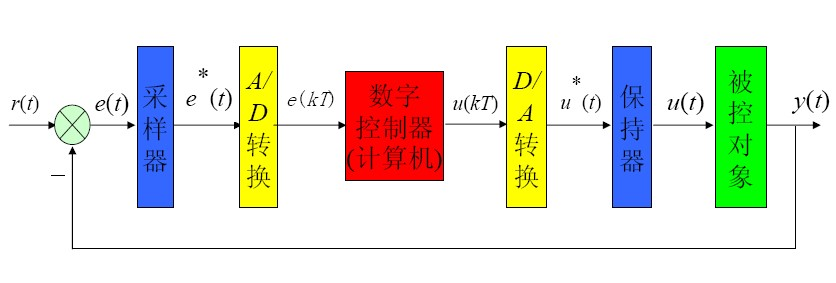
\includegraphics[width=0.6\textwidth]{fig_3_01}\\
  \caption{典型的计算机控制系统的结构}\label{fig_3_01}
\end{figure}


\begin{figure}[h]
  \centering
  % Requires \usepackage{graphicx}
  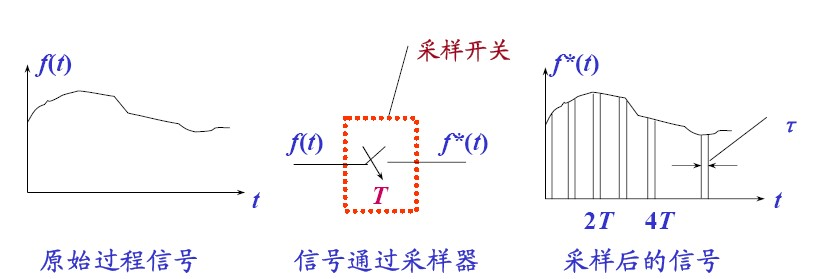
\includegraphics[width=0.6\textwidth]{fig_3_02}\\
  \caption{过程连续信号采样过程示意图}\label{fig_3_02}
\end{figure}

时域描述:

\begin{eqnarray}
% \nonumber to remove numbering (before each equation)
  f_s &=& \frac{1}{T} \\
  \omega_s &=& \frac{2\pi}{T}=2\pi f_s
\end{eqnarray}

其中,采样周期T(s),
闭合时间$\tau$(s),
采样角频率$\omega_s$(rad/s),
采样频率$f_s$(Hz)。



理想的单位脉冲函数为:

\begin{displaymath}
\left\{ \begin{array}{ll}
\delta(t)=\infty, & \textrm{for $t=0$}\\
\delta(t)=0 & \textrm{for $t\neq 0$}\\
\int_{-\infty}^{+\infty} \delta(t)dt=1 &
\end{array} \right.
\end{displaymath}

设$\delta (t-kT)$ 是$t=kT$时刻的理想采样脉冲,则

\begin{equation}
  f^*(t)=f(t)\sum_{k=0}^\infty\delta(t-kT)
\end{equation}


因为$f^*(t)$只与$f(t)$在脉冲出现瞬间的值 $f(kT)$有关,故采样信号可用下式表示:

\begin{equation}
  f^*(t)=f(t)\sum_{k=0}^\infty f(kT)\delta(t-kT) = f(t)\delta_T(t)
\end{equation}



\subsection{采样定理}


对于连续信号$f(t)$,记其傅立叶变换为$F(j\omega)$。则对于离散后的采样信号$f^*(t)$,其傅立叶变换后,为:

\begin{equation}
  F^*(j\omega)=\frac{1}{T}\sum_{k=-\infty}^{+\infty}F(j\omega-jk\omega_s)
\end{equation}

由上式可知,$F^*(j\omega)$由$F(j\omega)$向两端无限延拓而成,且幅值上相差$\frac{1}{T}$。此时,$\omega_s$与$\omega_{max}$的大小关系就对$F^*(j\omega)$的形态产生影响,如图\ref{fig_3_03}所示。


\begin{figure}[h]
  \centering
  % Requires \usepackage{graphicx}
  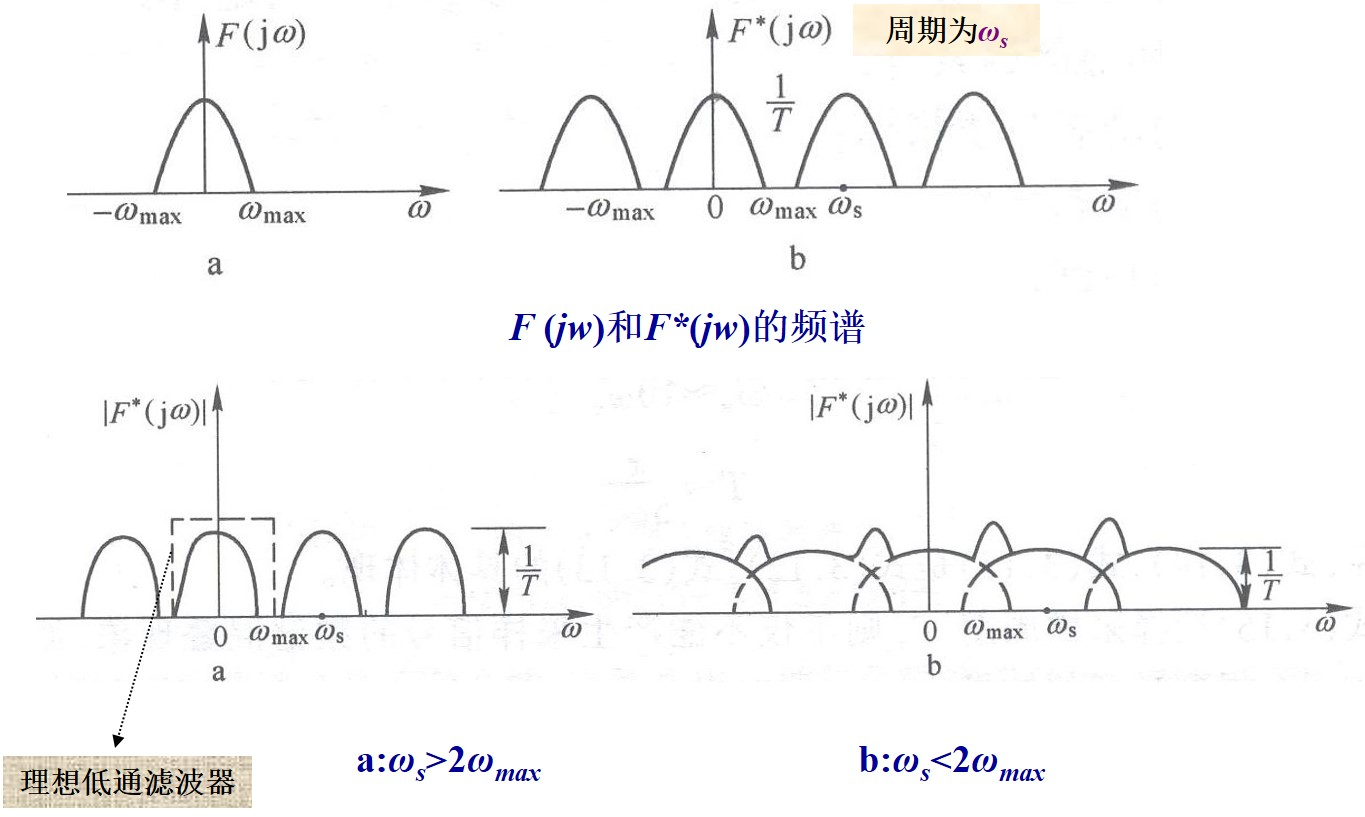
\includegraphics[width=0.6\textwidth]{fig_3_03}\\
  \caption{采样信号频谱的两种情况}\label{fig_3_03}
\end{figure}






\begin{remark}

 \textbf{香农采样定理}:一个连续时间信号$f(t)$,设其频带宽度是有限的,其最高频率为$\omega_{max}$(或$f_{max}$)。如果在等间隔点上对该信号$f(t)$ 进行连续采样,为了使采样后的离散信号$f^*(t)$ 能包含原信号$f(t)$的全部信息量,则采样角频率必须满足以下关系:

$\omega_{s}\ge2\omega_{max}$ 或者 $T_s\le \frac{T_{max}}{2}$

采样后的离散信号$f^*(t)$才能无失真地复现$f(t)$。

其中,$\omega_s=2\pi f_s=\frac{2\pi}{T_s}$

\end{remark}





\subsection{采样频率的选择}

常见过程参数的采样周期T,如图\ref{fig_3_04}所示。

\begin{figure}[h]
  \centering
  % Requires \usepackage{graphicx}
  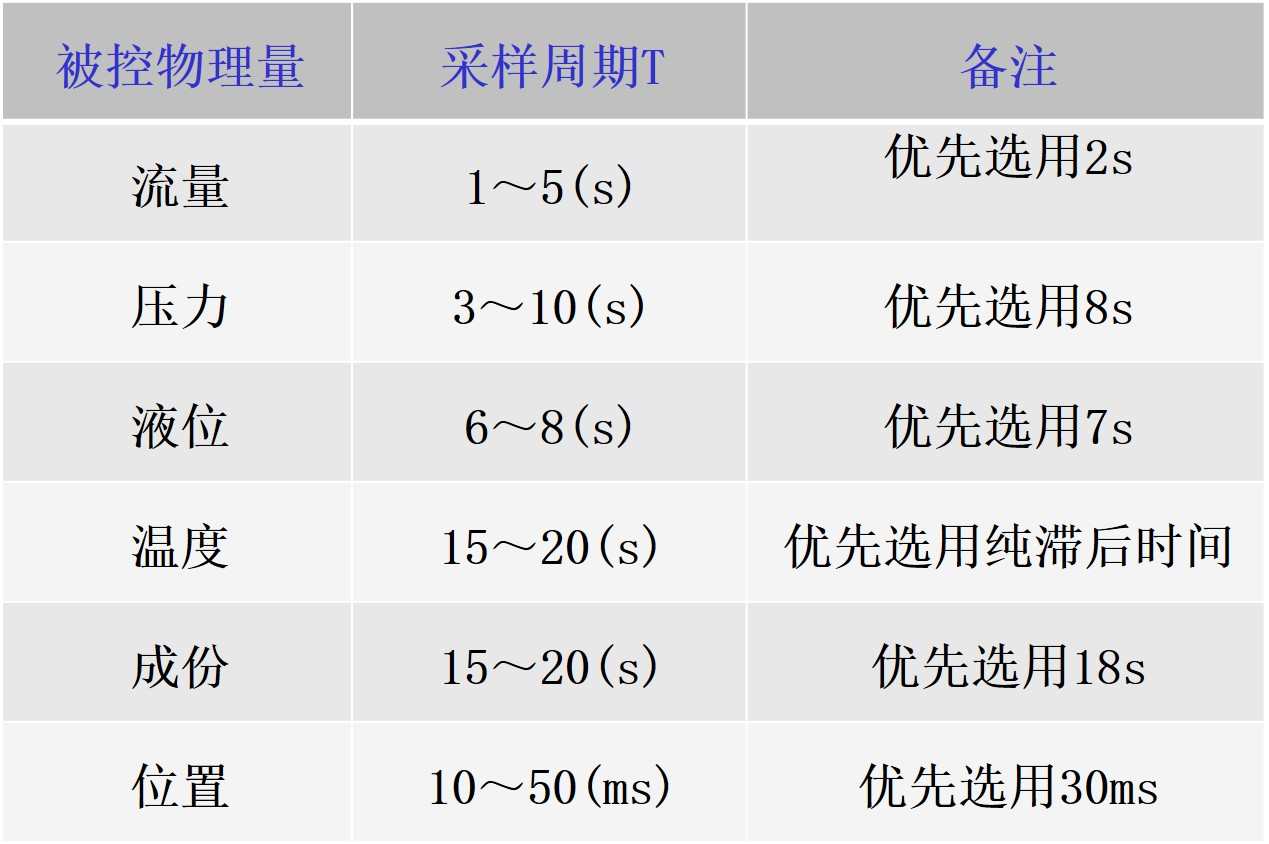
\includegraphics[width=0.4\textwidth]{fig_3_04}\\
  \caption{采样周期的选取}\label{fig_3_04}
\end{figure}





\section{线性化处理}


计算机从工程输入通道得到的现场信号与该信号所代表的对应的物理量之间不一定是线性关系,经常存在着非线性关系。
例如,在温度测量中,常用的Pt100铂电阻,其适用范围为(-200℃,850℃)。根据IEC 标准751-1983规定,Pt100铂电阻的阻值与温度的关系为


\begin{displaymath}
\left\{ \begin{array}{ll}
R_t = R_0[1+At+Bt^2+C(t-100)t^3], & \textrm{$-200\le t \le 0$}\\
R_t = R_0[1+At+Bt^2], & \textrm{$0 < t \le 850$}
\end{array} \right.
\end{displaymath}

再如在流量测量中,孔板测量气体或液体的流量,差压变送器输出的孔板差压信号ΔP,同实际流量F之间成平方根关系,即:

\begin{equation}
  F=K\sqrt{\Delta P}
\end{equation}
式中,K 是流量系数,也是非线性关系。

非线性补偿的三种方法:

\begin{enumerate}
  \item 公式计算法:适用于解析式明确的非线性函数关系;
  \item 查表法;
  \item 线性插值法,即:
  \begin{equation}
y=y_i+\frac{y_{i+1}-y_i}{x_{i+1}-x_i}(x-x_i)
\end{equation}
\end{enumerate}




\section{标度变换}

\textbf{标度变换}:测量值(进入计算机的二进制)与工程值的转换(实际温度、压力、流量)。\textbf{目的}:为了进行显示、记录、打印以及报警,必须将数字量转换成不同量纲,以便操作人员进行监视和管理生产。






\subsection{线性参数标度变换}

一般可采用以下公式进行变换:

\begin{equation}
A_x=\frac{N_{X}-N_0}{N_{M}-N_0}(A_M-A_0)+A_0
\end{equation}

例:某热处理炉温度测量表的量程为200到800摄氏度。在某一时刻,计算机采样并经数字滤波后的数字量为CDH,求此时对应的温度。

解:略。

\subsection{非线性参数标度变换}

(一)如被测量为非线性刻度时,其标度变换应具体分析,如:流量测量中,其流量与差压的公式为:
\begin{equation}
  F=K\sqrt{\Delta P}
\end{equation}

      测量流量时的标度变换公式为:
\begin{equation}
\frac{G_X-G_0}{G_M-G_0}=\frac{K\sqrt{\Delta N_X}-K\sqrt{\Delta N_0}}{K\sqrt{\Delta N_M}-K\sqrt{\Delta N_0}}
\end{equation}

(二)线性化处理

级数展开法:该方法的思想是利用泰勒级数展开把一些计算机基本指令集不包含的数学运算转换为更为便捷的乘加运算。例如,$y=\sqrt{x}$在$x=1$附近的级数展开为:

\begin{equation}
y=\sqrt{x}=1+\frac{1}{2}(x-1)-\frac{1}{8}(x-1)^2+\frac{1}{16}(x-1)^3+\ldots
\end{equation}

线性化处理还可通过迭代法实现,常用的有牛顿迭代法。迭代公式依据原计算公式而确定。上式所对应的牛顿迭代公式为:

\begin{equation}
y_{k+1}=\frac{1}{2}(y_{k}+\frac{x}{y_{k}})
\end{equation}



\section{越限报警处理}

超限报警分为上限报警、下限报警及上下限报警。

\begin{enumerate}
  \item 上限报警��

       若Xn>Xmax,则上限报警,否则继续执行原定操作。
  \item 下限报警��

      若Xn<Xmin,则下限报警,否则继续执行原定操作。��
  \item 上下限报警��

      若Xn>Xmax,则上限报警,否则对下式作判别:Xn<Xmin?若是,则下限报警,否则继续原定操作。
\end{enumerate}

图\ref{fig_3_05}为简单的上下限报警流程图。图\ref{fig_3_06}为考虑越限次数的报警流程图。
\begin{figure}[h]
  \centering
  % Requires \usepackage{graphicx}
  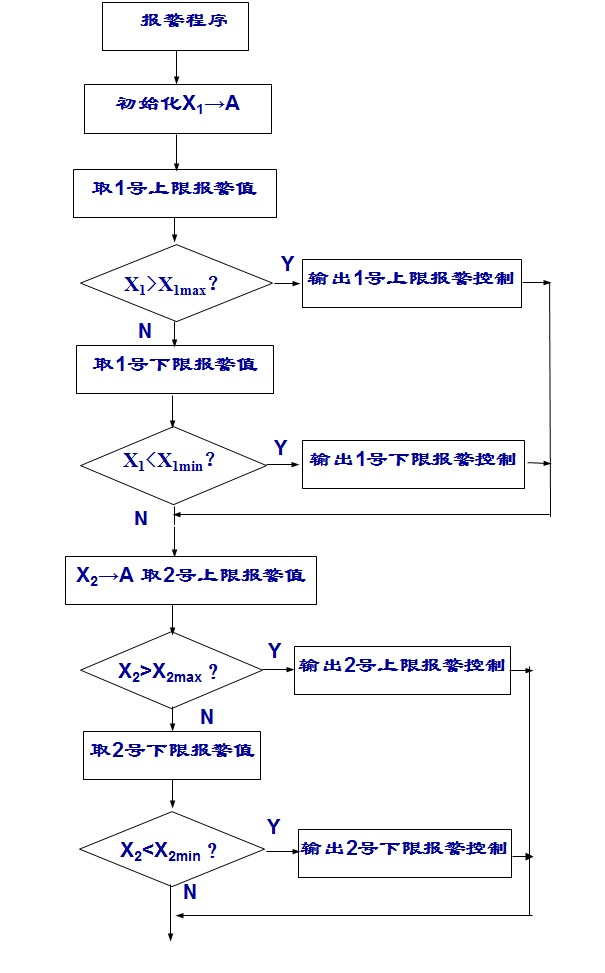
\includegraphics[width=0.4\textwidth]{fig_3_05}\\
  \caption{简单的上下限报警流程图}\label{fig_3_05}
\end{figure}

\begin{figure}[h]
  \centering
  % Requires \usepackage{graphicx}
  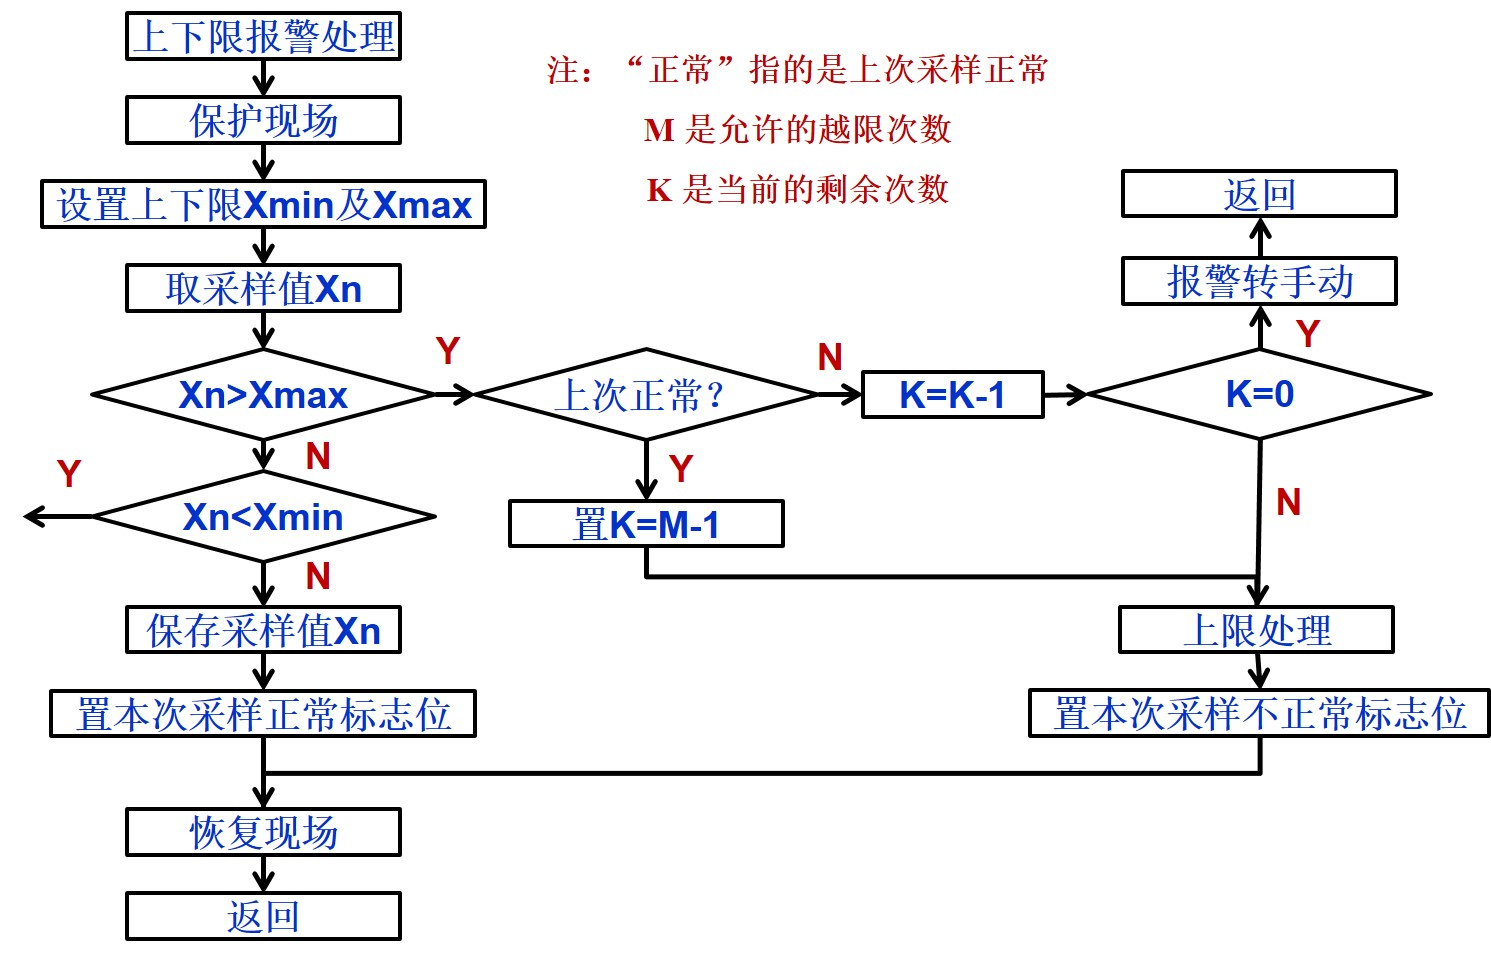
\includegraphics[width=0.7\textwidth]{fig_3_06}\\
  \caption{考虑越限次数的报警流程图}\label{fig_3_06}
\end{figure}




\section{数字滤波技术}

实质上它是一种程序滤波。  数字滤波克服了模拟滤波器的不足,它与模拟滤波器相比,有以下几个优点:
\begin{itemize}
  \item 数字滤波是用程序实现的,可多个通道公用一个滤波程序;

  \item 不需要增加硬设备,所以可靠性高,稳定性好,不存在各个回路之间的阻抗匹配问题;

  \item 数字滤波可以对很低的频率进行滤波;

  \item 数字滤波器可根据信号的不同,采用不同的滤波方法或滤波参数,具有灵活、方便、功能强的特点。

\end{itemize}


\subsection{程序判断滤波方法}

(1)限幅滤波—消除幅度较大的尖峰干扰

如果$|Y_n-Y_{n-1}|\le \Delta y$,则取$Y_n$; 如果$|Y_n-Y_{n-1}|> \Delta y$,则取$Y_{n-1}$。

(2)限速滤波—消除高频干扰

如果$|Y_2-Y_{1}|\le \Delta y$,则取$Y_2$; 如果$|Y_2-Y_{1}|> \Delta y$,则存$y_2$,采$Y_{3}$;
如果$|Y_3-Y_{2}|\le \Delta y$,则取$Y_3$; 如果$|Y_3-Y_{2}|> \Delta y$,则取$({Y_{2}+Y_{3}})/2$;


\begin{remark}
程序判断滤波法

  A、方法:根据经验判断,确定两次采样允许的最大偏差值(设为A),每次检测到新值时判断:如果本次值与上次值之差<=A,则本次值有效。如果本次值与上次值之差>A,则本次值无效,放弃本次值,用上次值代替本次值

  B、优点:能有效克服因偶然因素引起的脉冲干扰。

  C、缺点:无法抑制那种周期性的干扰,平滑度差。
\end{remark}

\subsection{中值滤波方法}

这种滤波法是将被测参数连续采样N次(一般N取奇数),然后把采样值按大小顺序排列,再取中间值作为本次的采样值。消除脉冲性质的干扰。
\begin{remark}
  中位值滤波法

A、方法:连续采样N次(N取奇数),把N次采样值按大小排列,取中间值为本次有效值。

B、优点:能有效克服因偶然因素引起的波动干扰,对温度、液位的变化缓慢的被测参数有良好的滤波效果。

C、缺点:对流量、速度等快速变化的参数不宜。

\end{remark}
\subsection{算术平均滤波}

\begin{equation}
\bar{Y_n} = \frac{1}{n}\sum_{i=0}^{n-1}x_i
\end{equation}

\begin{remark}
  算术平均滤波法

  A、方法:连续取N个采样值进行算术平均运算。N值较大时:信号平滑度较高,但灵敏度较低;N值较小时:信号平滑度较低,但灵敏度较高。N 值的选取:一般流量,N=12;压力:N=4

  B、优点:适用于对一般具有随机干扰的信号进行滤波,这样信号的特点是有一个平均值,信号在某一数值范围附近上下波动。

  C、缺点:对于测量速度较慢或要求数据计算速度较快的实时控制不适用,比较浪费RAM。
\end{remark}

\subsection{加权平均滤波}

\begin{equation}
\bar{Y_n} = \sum_{i=0}^{n-1}C_ix_i
\end{equation}
其中,
\begin{equation}
 \sum_{i=0}^{n-1}C_i =1
\end{equation}

\begin{remark}
  相对于算术平均滤波,加权平均滤波可以适当修改各采样点的权重。例如,增加新采样数据的权重,使滤波结果更能显现数据最近的变化趋势。
\end{remark}



\subsection{一阶滞后滤波(惯性滤波方法)}
慢速随机变量,短时间内连续采样。如图\ref{fig_3_07}所示,其传递函数为:

\begin{equation}
  G(s)=\frac{X(s)}{U(s)}=\frac{1}{1+T_fs}
\end{equation}
其中:$T_f=RC$为滤波器的时间 常数。

\begin{equation}
T_f\frac{x(k)-x(k-1)}{T}+x(k)=u(k)
\end{equation}

令$\alpha = T_f/(T_f+T)$,则有

\begin{equation}
x(k)=(1-\alpha)u(k)+\alpha x(k-1)
\end{equation}




\begin{figure}
  \centering
  % Requires \usepackage{graphicx}
  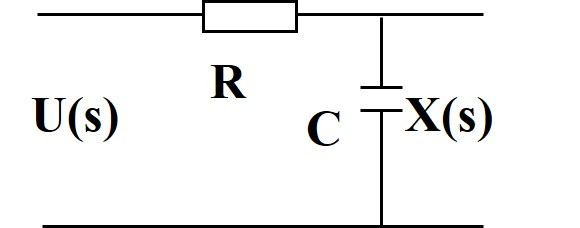
\includegraphics[width=0.34\textwidth]{fig_3_07}\\
  \caption{一阶滞后滤波}\label{fig_3_07}
\end{figure}


\begin{remark}
  一阶滞后滤波法

  优点:对周期性干扰具有良好的抑制作用,适用于波动频率较高的场合。

  缺点: 相位滞后,灵敏度低,滞后程度取决于a值大小,不能消除滤波频率高于采样频率的1/2的干扰信号。
\end{remark}

\subsection{复合数字滤波}

复合滤波就是把两种以上的滤波方法结合起来使用。例如把中值滤波的思想与算术平均的方法结合起来,就是一种常用的复合滤波法。具体方法是首先将采样值按大小排队,去掉最大和最小的,然后再把剩下的取平均值。这样显然比单纯的平均值滤波的效果要好。


例:一阶滞后滤波加上算术平均值滤波的复合滤波子程序,流程图如图\ref{fig_3_08}所示。其中,主程序初始化中已对X、S和a初始化。

\begin{figure}
  \centering
  % Requires \usepackage{graphicx}
  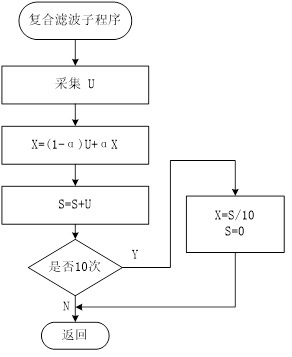
\includegraphics[width=0.45\textwidth]{fig_3_08}\\
  \caption{复合滤波器}\label{fig_3_08}
\end{figure}




\section{本章要点总结}


\begin{itemize}
  \item 什么是线性化处理?线性化方法有几种?

  \item 理解标度变换;

  \item 了解超限报警的类型和方法;

  \item 数字滤波的特点,有几种常用的数字滤波方法?各有何特点?

\end{itemize}
